\chapter{\xlabel{pol2_dr}POL-2 Data Reduction - The Theory}
\label{sec:dr}
\section{\xlabel{dataflow}The Data Flow}

POL-2 data reduction is a complex and involved process
for which a broad overview is presented first before
the specific details are discussed.


\begin{figure}[t!]
\begin{center}
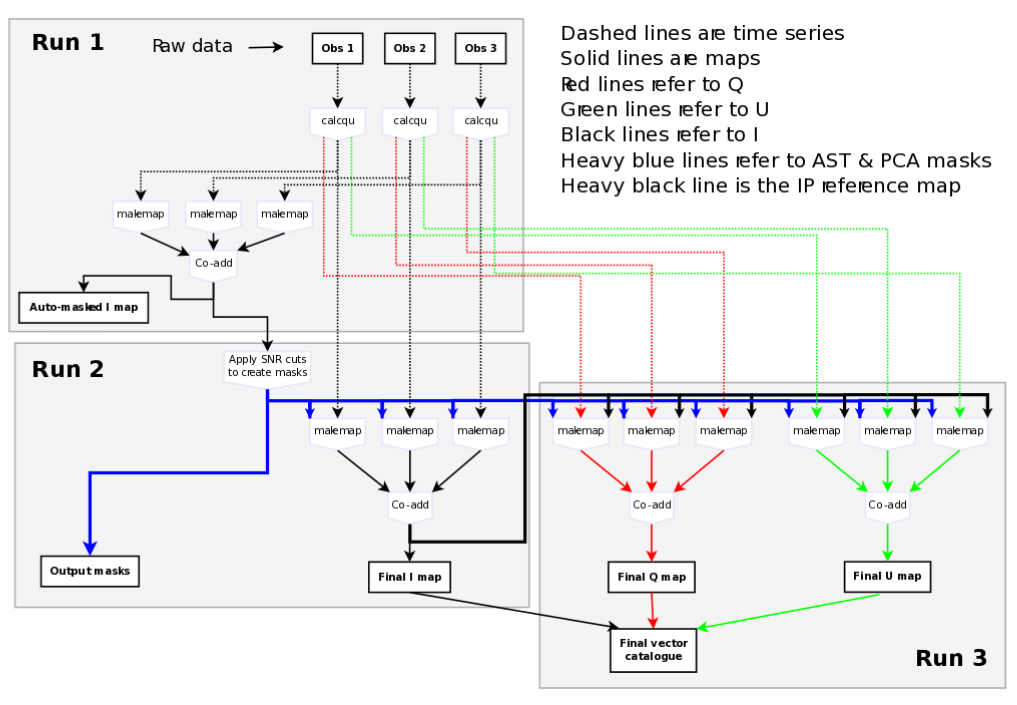
\includegraphics[width=0.95\linewidth]{pol2-dr-flow.png}
\label{fig:pol2drflow}
\caption [POL-2 Data Flow]{
  \small The data flow of the POL-2 data reduction method is
  presented. In this example three POL-2 observations are
  reduced and combined in various stages and combination to
  produce I, Q and U maps.
}
\end{center}
\end{figure}

\subsection*{Step 1}

\subsection*{Step 2}

\subsection*{Step 3}



\section{\xlabel{makemap}Makemap}

The POL-2 data reduction builds upon the SCUBA-2 make-map data reduction. The Dynamic Iterative Map-Maker, hereafter just referred to as the map-maker is the tool you will use to produce SCUBA-2 maps, and is implemented by the Smurf makemap command. It performs all pre-processing steps to clean the data, followed by solving for multiple signal components using an iterative algorithm, and binning the resulting time-series data to produce a final science map. 

\cite{smurf}

\section{\xlabel{pca}PCA}


\section{\xlabel{masking}Masking}


\section{\xlabel{addingdata}Adding new observations}



\section{\xlabel{tailoredDR}Tailoring your reduction}

\subsection*{variances between POL-2 maps}

MAPVAR is a parameter that controls the variances in the coadded 
I, Q and U maps are formed.

If  MAPVAR is set TRUE, the variances in the coadded I, Q and U maps
are formed from the spread of pixel data values in the individual
observation maps. If MAPVAR is FALSE (the default), the variances in
the coadded maps are formed (as in previous versions of pol2map) by
propagating the pixel variance values created by makemap from the
individual observation maps.

Only use MAPVAR=TRUE if you have enough observations to
make the variances between them meaningful. It's hard to put a lower
limit on it, but it is advised that at a minimum 10 observations.


If you want to test the effect of this option on a field for which you
already have the I, Q and U maps from a set of individual
observations, you can do the following:

\begin{terminalv}
% pol2map in=maps/\* iout=imapvar qout=qmapvar uout=umapvar mapvar=yes \
                   ipcor=no cat=cat_mapvar debias=yes
\end{terminalv}

assuming your I, Q and U maps are in directory "maps". The variances
in imapvar.sdf qmapvar.sdf and umapvar.sdf will be calculated using
the new method, and these variances will then be used to form the
errors in the cat_mapvar.FIT catalogue.



